\chapter{Coding}\label{ch:coding}


\begin{figure}[htp]
    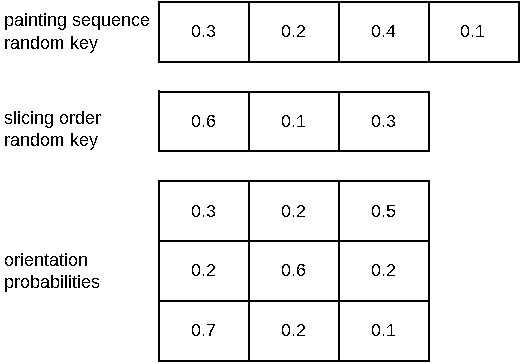
\includegraphics[width=1.0\textwidth, center]{chromosome}\label{fig:chromosome}
    \caption{
        Example of an individual representation – 3D chromosome composed of two random key vectors
        and one matrix, whose rows are also random keys.
        Each vector and matrix row form a probability distribution, i.e., they sum up to 1.
    }
\end{figure}

\begin{figure}[htp]
    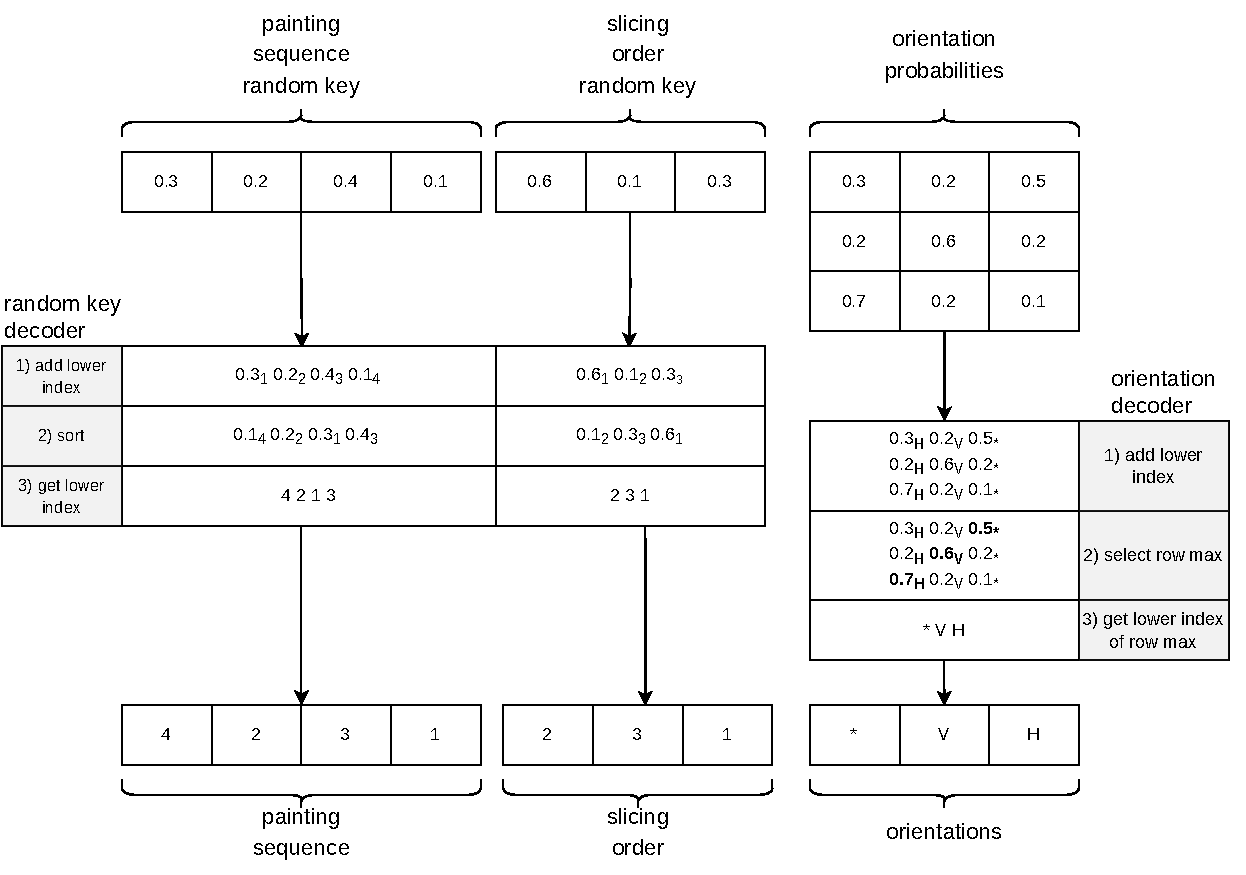
\includegraphics[width=1.1\textwidth, left]{individual_decoding}
    \caption{
        Individual decoding example. Both the painting sequence random key and slicing order random key
        are decoded using the same procedure. The decoded individual can be used to construct a slicing layout.
    }
    \label{fig:individual-decoding}
\end{figure}

\begin{figure}[htp]
    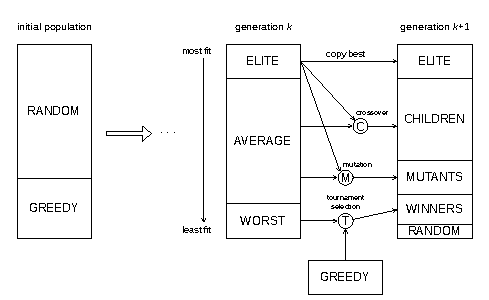
\includegraphics[width=1.1\textwidth, left]{pupulation_schema}\label{fig:population-schema}
    \caption{Initial population generation strategy and transition from generation $k$ to $k+1$.}
\end{figure}


\section{Operators}\label{sec:operators}
This sections describes operators – actions on the individual representation
seen in section~\ref{subsec:individual-representation}.

We can guide the genetic search in two basic ways – diversification and intensification.
If the diversification is high, the search process is biased towards exploring genomes
that may be vastly different from the one already present in the population.
This tries to prevent the genetic search from getting stuck in a local optimum.
Diversification that is too high would reassemble a random walk, ultimately randomly sampling
from the space of all possible genomes. On the other hand, if the intensification is high,
biased towards exploiting similar genemos takes precedence.

It is crucial to find the correct balance between diversification and intensification.
One way to control the diversification in genetic algorithm is setting
mutation probability – high chance of mutation means higher diversification, low change is the opposite.
Intensification can be similarly controller by the crossover probability.
\ref{TODO}

\subsection{Mutation}\label{subsec:mutation}
Mutation takes place on all 3 parts of a chromosome, as seen in example in table \ref{tab:ind-rep-example}.
Since both random keys vectors and orientation probabilities form a probability distribution vector,
it is easy to perform mutation by replacing a value with a randomly generated one from interval $[0,1]$
and then normalize back to the probability distribution.

For example, consider $$[0.6, 0.1, 0.3]$$ be a painting sequence random key or slicing order random key.
Mutation operator would randomly choose one position in the vector, say the first one, and replace it
with a randomly generated one from interval $[0,1]$. The result may be $$[0.9, 0.1, 0.3]$$.
The mutated vector forms no longer a probability distribution and to obtain the mutated value
it needs to be normalized – finally ending up with $[0.7, 0.07, 0.23]$.

Mutation for the orientation probabilities is the same but with the first additional
step of randomly choosing which of the probability vectors will undergo the aforementioned process.

\begin{figure}[htp]
    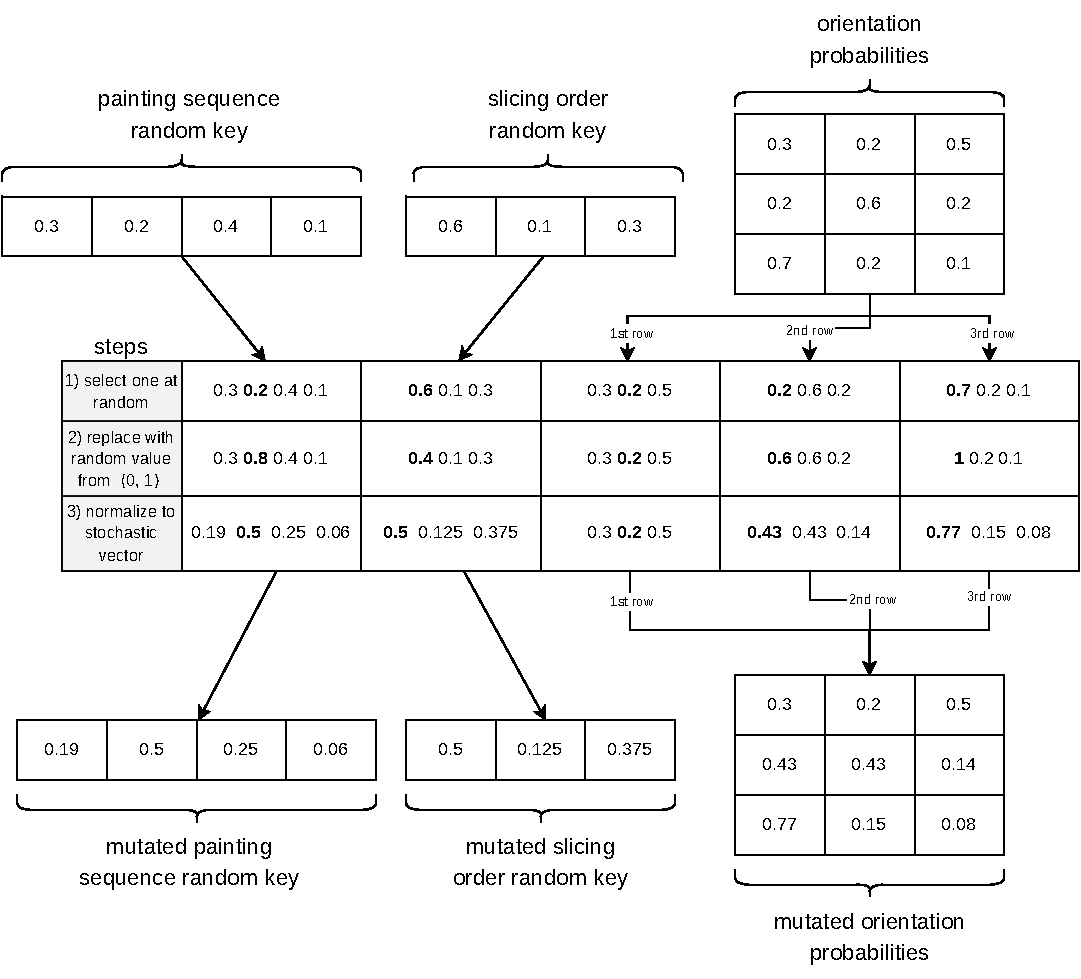
\includegraphics[width=1.0\textwidth, left]{muation}\caption{
        Example of a mutation on all three parts of a chromosome.
        Since all parts can be treated as a random key, only one procedure
        is used – replace one value at random and then normalize to a stochastic vector.
    }
    \label{fig:mutation}
\end{figure}

\subsection{Crossover}\label{subsec:crossover}

\begin{figure}[htp]
    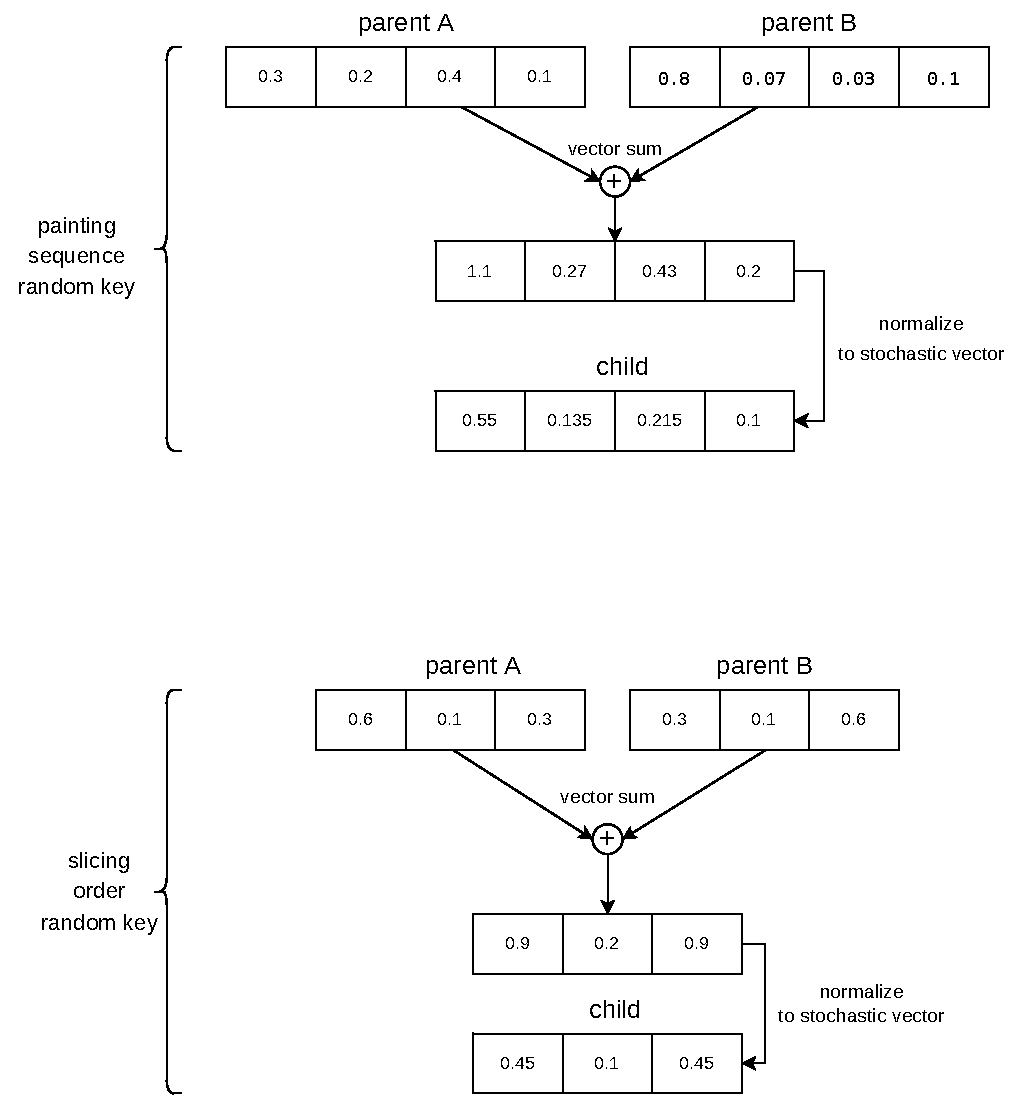
\includegraphics[width=1.1\textwidth, left]{crossover_random_keys}\caption{
        Crossover example for painting sequence and slicing order random keys.
        The procedure is the same for both – sum parent vectors and then normalize to stochastic vector.
    }
    \label{fig:crossover-random-keys}
\end{figure}

\begin{figure}[htp]
    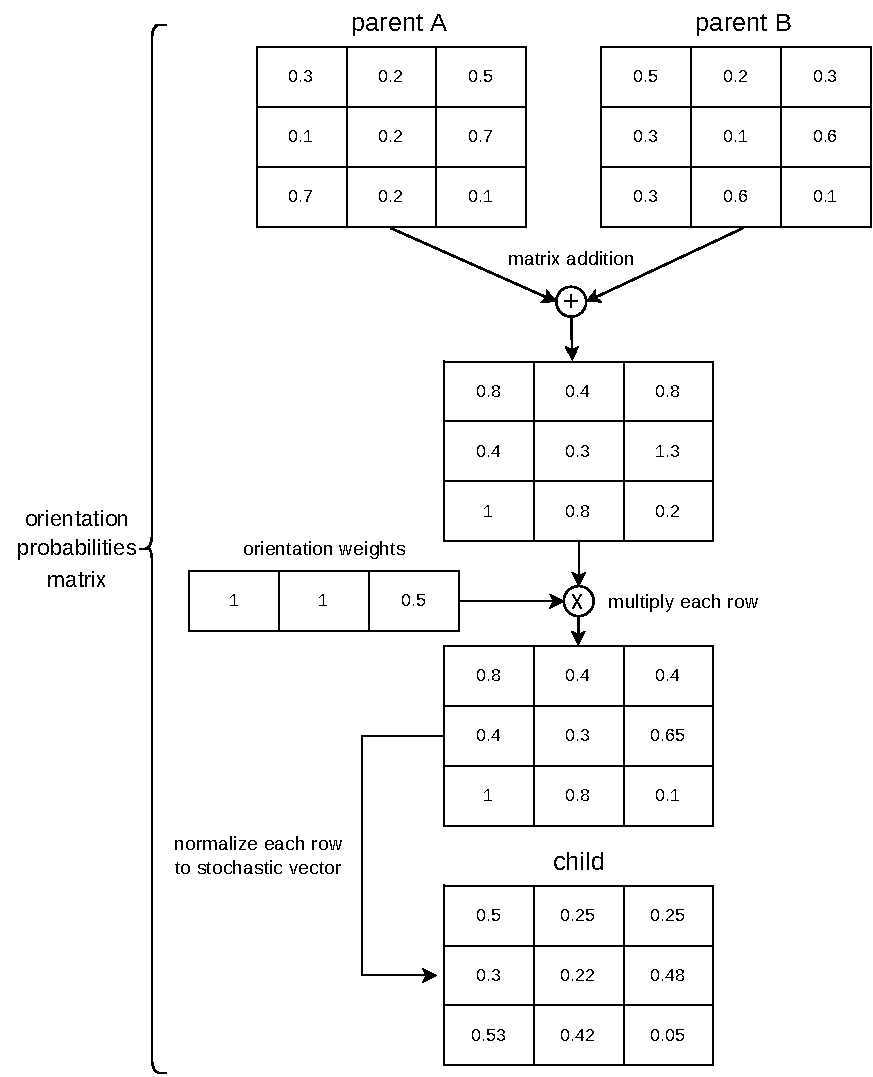
\includegraphics[width=0.85\textwidth, left]{crossover_orientation_probabilities}\caption{
        Crossover example for orientation probabilities. The procedure is first to sum parent matrices,
        then weight each row with orientation weights and normalize each row to a stochastic vector.}
    \label{fig:crossover-orientation-probabilities}
\end{figure}


